\documentclass{article}[12pt]
\renewcommand{\baselinestretch}{1.5}

\usepackage[affil-it]{authblk}
\usepackage[space]{grffile}

\usepackage[a4paper]{geometry}
\geometry{verbose}
\usepackage{float}
\usepackage{graphicx}
\usepackage{setspace}

\usepackage[utf8]{inputenc}
\usepackage[english]{babel}

\usepackage{latexsym,textcomp,longtable,tabulary}
\usepackage{booktabs,array,multirow}
\usepackage{amsfonts,amsmath,amssymb,mathbbol,calc}
\usepackage{subfigure,color,blindtext,enumitem,siunitx}

\usepackage{mathtools}
\usepackage{url,hyperref,etoolbox}
\numberwithin{equation}{section}
\hypersetup{colorlinks=false,pdfborder={0 0 0}}

%+figure layout options
\restylefloat{figure}
\setlist{leftmargin=*,before=\setlength{\rightmargin}{\leftmargin}}
%-figure layout options

\providecommand\citet{\cite}
\providecommand\citep{\cite}
\providecommand\citealt{\cite}


\makeatletter
\makeatother


\newif\iflatexml\latexmlfalse
\providecommand{\tightlist}{\setlength{\itemsep}{0pt}\setlength{\parskip}{0pt}}%
\AtBeginDocument{\DeclareGraphicsExtensions{.pdf,.PDF,.eps,.EPS,.png,.PNG,.tif,.TIF,.jpg,.JPG,.jpeg,.JPEG}}
\begin{document}

\title{
On the affect of the Laplacian in equlibration
dynamics of the Spherical Model
}

\author{Gregory Szep}
\affil{King's College London}
\date{\today}

\maketitle
Consider a system of $N$ linearly interacting degrees of freedom. We collect
them into a vector $\mathbf{\bar{s}}(t) = \left(\,s_1(t),\cdots, s_N(t)\,\right)$
and represent their interactions with random coupling matrix $\mathbf{J}(t)$.
We subject them to a global constraint: lying on an $N$-dimensional sphere of
radius $N$, enforced by lagrange multiplier $\mu$. We write down the
Langevin Equation of motion with external noise $\boldsymbol\xi(t)$, dropping
the explicit time dependence for brevity.
\begin{gather}
\partial_t\mathbf{\bar{s}} = (\mathbf{J}-\mu)\mathbf{\bar{s}}+\boldsymbol\xi\quad\\
\text{where}\quad\mu = \frac{1}{N}\mathbf{\bar{s}}^{\top}\left(\mathbf{J}\mathbf{\bar{s}}+\boldsymbol\xi\right)\quad\text{enforces constraint}\quad|\mathbf{\bar{s}}(t)|^2=N
\end{gather}
The following is an attempt to characterise the statistical differences between
spatial and non-spatial interactions, and their effect on the equilibration
dynamics by introducting the discretised Laplacian $\Delta$ as a diffusive term.

\section{Analytical Solutions}
Here we follow the methods used to obtain exact solutions\cite{} in the
field theoretic setting of the model.
\begin{align*}
  \mathbf{\bar{u}}(t)=\mathbb{e}^{\mathbf{\Lambda}t}\mathbf\Gamma^{1/2}\mathbf{\bar{u}}(0)
\end{align*}
\subsection{Spectra of Discrete Laplacians}
Using the Circular Diagonalization Theorem~\cite{} one can derive the
eigenvalues $\lambda_N(k)$ of an $N\times N$ matrix $\mathbf X$ which
represents the second-order central difference approximation to the
second derivative along $N$ sites of a one dimensional ring of unit
circumference.
\begin{align}
  \mathbf X :=
  \begin{pmatrix}
    -2 & 1 &  &  &  & 1 \\
    1 & -2 & 1 &  &  &  \\
    & 1 & \ddots & \ddots &  & \\
    & & \ddots & \ddots & 1 & \\
    & & & 1 & -2 & 1 \\
    1 & & & & 1 & -2 \\
  \end{pmatrix}\\
  \begin{matrix}
    \lambda_N(k)=2\left(\cos\left(\frac{2\pi k}{N}\right)-1\right) \\
    k\in\{0,1,\cdots,N-1\}
  \end{matrix}
  \qquad
\end{align}
As the number of sites $N\rightarrow\infty$ the argument $k/N\in[0,1]$
and the eigenvalues remain bounded $-2<\lambda<0$. By shifting and scaling
the index $k\rightarrow\frac{k-N\pi}{2\pi}$ the eigenvalues are expressed as
the familiar dispersion relation~\cite{}.
\begin{align}
  \lambda(x)&=
  -2\left(\cos x+1\right)
  \quad x\in[-\pi,\pi]
\end{align}
The discrete $M$-dimensional laplacian is simply the kronecker sum of one
dimensional cases $\mathbf\Delta=\mathbf X\oplus\mathbf X\oplus\cdots\oplus\mathbf X$
and thus its eigenvalues is simply the sum one dimensional dispersions~\cite{}.
\begin{align}
  \lambda(\mathbf{\bar{x}})&=
  -2\sum_{x\in\mathbf{\bar{x}}}\left(\cos x+1\right)
  \quad \mathbf{\bar{x}}\in[-\pi,\pi]^M
\end{align}
The probability density $\rho(\lambda)$ can be expressed as an integral
over the region $\Omega=[-\pi,\pi]^M$ in complete analogue with the
density of states.
\begin{align*}
  \rho(\lambda')&=\frac{1}{Z_M}\int_{\Omega}\!\delta(\lambda'-\lambda(\mathbf{\bar{x}}))\,\mathrm{d}\mathbf{\bar{x}}
\end{align*}
We proceed with an element-wise change of variables $\mathbf{\bar{u}}=2\cos \mathbf{\bar{x}}$ and
recognise that the integration region is $M$-fold symmetric across each
component axis, which allows restrict the domain of integration to a
hyperoctant. Thus in the new coordinates $\mathbf{\bar{u}}$ the
$M$-dimensional hypercube region becomes $\Omega'=[-2,2]^M$.
\begin{align*}
  \rho(\lambda)&=\frac{1}{Z_M}
  \int_{\Omega'}\!
  \frac{\delta(\Lambda_M+\sum_{u\in\mathbf{\bar{u}}}u)}
  {\sqrt{\prod_{u\in\mathbf{\bar{u}}}(1-u^2/4) }}
  \,\mathrm{d}\mathbf{\bar{u}}
  \qquad
  \begin{matrix}
    \Lambda_M=\lambda+2M \\
    |\Lambda_M|\leq2M
  \end{matrix}
\end{align*}
The tricky aspect of this integral writing down how the domain of integration
$\Omega'\rightarrow\partial\Omega'(\Lambda_M)$ becomes of a function of $\Lambda_M$
after using the delta function filtering property.
\begin{figure}[H]
\centering{}
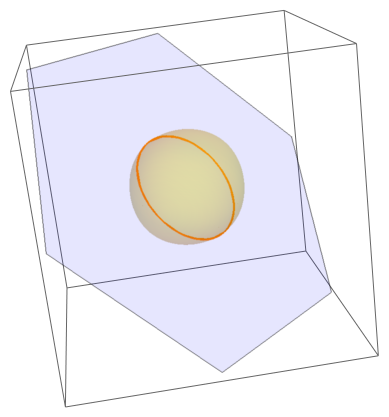
\includegraphics[scale=0.4]{figures/dos1}
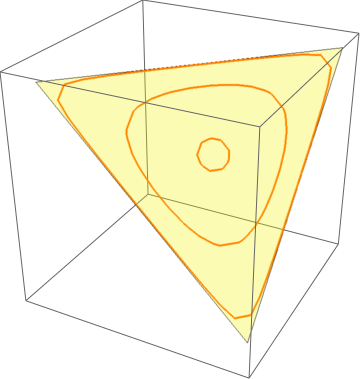
\includegraphics[scale=0.4]{figures/dos2}
\caption{Isosurfaces of the integrand $M=3$ within the cubic integration
region $\Omega'$ with delta constraint represented by a plane shifted from
the origin by parameter $\Lambda_3$. This illustration }
\label{fig:dos}
\end{figure}
\end{document}
